\begin{pastexam}[label={px:ncku-106-cce-ds-05}]{成大電通所 106 學年度 第二大題第 1 題}
（簡答；20 分）

\textbf{(20 pts)} Give a table which characterizes the priority of the operators.

\begin{center}
\begin{tabular}{|p{3.5cm}|p{2.2cm}|p{2.2cm}|}
\hline
priority & ISP & ICP \\ \hline
( & & 0 \\ \hline
! & 1 & 1 \\ \hline
* \quad / \quad \% & 2 & 2 \\ \hline
+ \quad - & 3 & 3 \\ \hline
= & 4 & 4 \\ \hline
( & 5 & \\ \hline
\end{tabular}
\end{center}

The expression is \quad (A + B) *( C - !D / E) \% F
\begin{enumerate}[label=\alph*.]
\item \textbf{(5 pts)} Show the equivalent postfix expression if we use a stack to evaluate the
postfix expression in C++ from left to right.
\item \textbf{(5 pts)} Based on a, please show the status of the stack in each time before you pop
data, how many pop operations you have to perform.
\item \textbf{(7 pts)} Draw a binary tree representation which corresponds to the sequence of its
infix expression.
\item (3 pts) Please show the results of the expression 5*2 +30 -20 -80/5 if we reverse the
priority of the operators * / with the priority of the operators + - and the evaluation of
operators of the same priority will proceed from right to left.
\end{enumerate}
\end{pastexam}

\begin{pastsoln}
表中數字\textbf{越小優先順序越高}（! 最高、= 最低）。 左括號讀進來時 ICP 是 $0$，一定會被 push；
進了堆疊 ISP 是 $5$，比所有運算子都低，不會被 pop 掉。 轉換規則：讀到運算子 $x$ 時，只要堆疊頂端的
ISP $\le$ $x$ 的 ICP，就 pop 出來寫到輸出，再把 $x$ push（資結書第~6.3.3~節的做法，只是數字大小的
方向相反）。 ISP 和 ICP 相等，所以同優先順序的運算子由左往右結合。 小題 d 的 $-$ 是減號。

\textbf{a.} 後序式：\texttt{A B + C D ! E / - * F \%}。

轉換過程（每讀一個符號後的輸出和堆疊，堆疊左邊是底）：
\begin{center}
\small
\begin{tabular}{cll}
\toprule
讀到 & 輸出 & 堆疊 \\
\midrule
( & & ( \\
A & A & ( \\
+ & A & ( + \\
B & A B & ( + \\
) & A B + & （pop 到左括號為止） \\
* & A B + & * \\
( & A B + & * ( \\
C & A B + C & * ( \\
- & A B + C & * ( - \\
! & A B + C & * ( - ! \\
D & A B + C D & * ( - ! \\
/ & A B + C D ! & * ( - /（頂端 ! 的 ISP $1 \le 2$，pop） \\
E & A B + C D ! E & * ( - / \\
) & A B + C D ! E / - & * \\
\% & A B + C D ! E / - * & \%（頂端 * 的 ISP $2 \le 2$，pop） \\
F & A B + C D ! E / - * F & \% \\
結束 & A B + C D ! E / - * F \% & \\
\bottomrule
\end{tabular}
\end{center}
讀到 $-$ 時頂端是左括號（ISP $5 > 3$），不 pop；讀到 $!$ 時頂端是 $-$（ISP $3 > 1$），不 pop。 對應
的完整括號式是 $((A + B) * (C - ((!D) / E))) \,\%\, F$。

\textbf{b.} 用堆疊計算後序式（資結書虛擬碼~6.7）：運算元就 push；二元運算子 pop 兩次（先取出的是
右運算元），一元的 ! pop 一次，算完把結果 push。 令 $T_1 = A + B$、$T_2 = !D$、$T_3 = T_2 / E$、
$T_4 = C - T_3$、$T_5 = T_1 * T_4$、$T_6 = T_5 \,\%\, F$。 每次 pop 之前的堆疊（左邊是底）：
\begin{center}
\small
\begin{tabular}{clll}
\toprule
第幾次 pop & 讀到 & pop 前的堆疊 & 取出 \\
\midrule
1 & + & A B & B \\
2 & + & A & A（push $T_1$） \\
3 & ! & $T_1$ C D & D（push $T_2$） \\
4 & / & $T_1$ C $T_2$ E & E \\
5 & / & $T_1$ C $T_2$ & $T_2$（push $T_3$） \\
6 & - & $T_1$ C $T_3$ & $T_3$ \\
7 & - & $T_1$ C & C（push $T_4$） \\
8 & * & $T_1$ $T_4$ & $T_4$ \\
9 & * & $T_1$ & $T_1$（push $T_5$） \\
10 & \% & $T_5$ F & F \\
11 & \% & $T_5$ & $T_5$（push $T_6$） \\
12 & 結束 & $T_6$ & $T_6$，即結果 \\
\bottomrule
\end{tabular}
\end{center}
五個二元運算子各 pop 兩次、! pop 一次，共 $11$ 次；最後再 pop 一次取出結果，總共 $12$ 次 pop。
（若最後只看頂端、不 pop，則是 $11$ 次。）

\textbf{c.} 運算式樹：內部節點是運算子，樹葉是運算元，中序走訪得到原來的中序式（資結書第~7.7~節）。
一元的 ! 只有一個子節點，放在右邊（中序時 ! 先印、再印 D，順序和原式一樣）。
\begin{center}
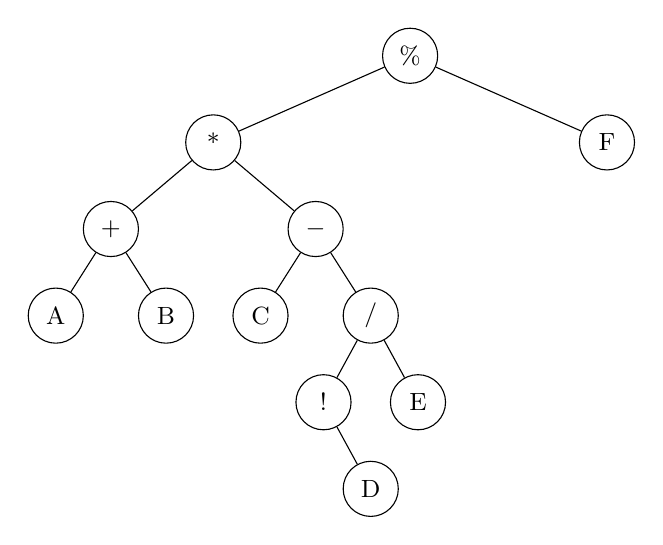
\begin{tikzpicture}[every node/.style={circle,draw,minimum size=7mm,inner sep=0pt,font=\small},
  level distance=11mm, level 1/.style={sibling distance=50mm}, level 2/.style={sibling distance=26mm},
  level 3/.style={sibling distance=14mm}, level 4/.style={sibling distance=12mm}]
\node {\%}
  child {node {*}
    child {node {+} child {node {A}} child {node {B}}}
    child {node {$-$}
      child {node {C}}
      child {node {/}
        child {node {!} child[missing] child {node {D}}}
        child {node {E}}}}}
  child {node {F}};
\end{tikzpicture}
\end{center}

\textbf{d.} 新規則：$+$、$-$ 比 $*$、$/$ 優先；同優先順序由右往左算。 所以先把 $+$、$-$ 連起來的
那一段 $2 + 30 - 20 - 80$ 算完，而且由右往左：
\[
2 + (30 - (20 - 80)) = 2 + (30 - (-60)) = 2 + 90 = 92 .
\]
剩下 $5 * 92 / 5$，同樣由右往左：$5 * (92 / 5)$。 用一般的數學除法，$92 / 5 = 18.4$，結果是
$5 \times 18.4 = 92$。 若照 C++ 的整數運算，$92 / 5 = 18$（捨去小數），結果是 $5 \times 18 = 90$。
（照原來的規則算是 $10 + 30 - 20 - 16 = 4$。）
\end{pastsoln}
